\documentclass[12pt]{article}
%\usepackage[utf8]{inputenc}
%\documentclass[UTF8]{ctexart}
%\usepackage[UTF8, heading = false, scheme = plain]{ctex}
\usepackage{geometry}
%geometry{a4paper,scale=0.9}
\geometry{a4paper,left=1cm,right=1cm,top=1cm,bottom=2cm}
\usepackage{amsfonts}
\usepackage{color}
\usepackage{url}
%\usepackage{biblatex}
\usepackage{amsmath}
\usepackage{amssymb}
\usepackage{latexsym}
\usepackage{listings}
\usepackage[usenames,dvipsnames]{xcolor}
\usepackage{cite}
%\addbibresource{ref.bib}
%\bibliography{ref.bib}
\usepackage{caption}
\usepackage{graphicx, subfig}
\usepackage{float}
%\usepackage[fontset=ubuntu]{ctex}
%\usepackage{fontspec}
\usepackage{xeCJK}
%\usepackage[colorlinks,
%anchorcolor=black,
%citecolor=black]{hyperref}
%\setmainfont{SimSun}
\usepackage[section]{placeins}
\usepackage{enumitem}
\usepackage{framed}
\usepackage[framemethod=TikZ]{mdframed}
\usepackage{indentfirst}
\usepackage{setspace}%使用间距宏包
\linespread{1.5}
\definecolor{mygreen}{rgb}{0,0.6,0}
\definecolor{mygray}{rgb}{0.5,0.5,0.5}
\definecolor{mybgray}{rgb}{0.95,0.95,0.95}
\definecolor{mymauve}{rgb}{0.58,0,0.82}
\lstset{
 backgroundcolor=\color{mybgray}, 
 basicstyle = \footnotesize,       
 breakatwhitespace = false,        
 breaklines = true,                 
 captionpos = b,                    
 commentstyle = \color{mygreen}\bfseries,
 extendedchars = false,             
 frame =shadowbox, 
 framerule=0.5pt,
 keepspaces=true,
 keywordstyle=\color{blue}\bfseries, % keyword style
 language = C++,                     % the language of code
 otherkeywords={string}, 
 numbers=left, 
 numbersep=5pt,
 numberstyle=\tiny\color{mygray},
 rulecolor=\color{black},         
 showspaces=false,  
 showstringspaces=false, 
 showtabs=false,    
 stepnumber=1,         
 stringstyle=\color{mymauve},        % string literal style
 tabsize=2,          
 title=\lstname                      
}

\title{题目汇总 I}
\author{leolinuxer}
%\date{June 2020}

\begin{document}
%\setlength{\parindent}{0pt}
\maketitle
\tableofcontents

\section{twoSum问题}
\url{https://github.com/labuladong/fucking-algorithm/blob/master/%E7%AE%97%E6%B3%95%E6%80%9D%E7%BB%B4%E7%B3%BB%E5%88%97/twoSum%E9%97%AE%E9%A2%98%E7%9A%84%E6%A0%B8%E5%BF%83%E6%80%9D%E6%83%B3.md}

\subsection{TwoSum I-基本形式}
这个问题的最基本形式是这样:给你一个数组和一个整数 target,可以保证数组中存在两个数的和为 target,请你返回这两个数的索引。

比如输入 nums = [3,1,3,6], target = 6,算法应该返回数组 [0,2],因为 3 + 3 = 6。

这个问题如何解决呢?首先最简单粗暴的办法当然是穷举了:

\begin{lstlisting}
int[] twoSum(int[] nums, int target) {

    for (int i = 0; i < nums.length; i++) 
        for (int j = i + 1; j < nums.length; j++) 
            if (nums[j] == target - nums[i]) 
                return new int[] { i, j };

    // 不存在这么两个数
    return new int[] {-1, -1};
}
\end{lstlisting}

这个解法非常直接,时间复杂度 $O(N^2)$,空间复杂度 $O(1)$。

可以通过一个哈希表减少时间复杂度:
\begin{lstlisting}
int[] twoSum(int[] nums, int target) {
    int n = nums.length;
    index<Integer, Integer> index = new HashMap<>();
    // 构造一个哈希表:元素映射到相应的索引
    for (int i = 0; i < n; i++)
        index.put(nums[i], i);
    
    for (int i = 0; i < n; i++) {
        int other = target - nums[i];
        // 如果 other 存在且不是 nums[i] 本身
        if (index.containsKey(other) && index.get(other) != i)
            return new int[] {i, index.get(other)};
    }
    
    return new int[] {-1, -1};
}
\end{lstlisting}

这样,由于哈希表的查询时间为 O(1),算法的时间复杂度降低到 O(N),但是需要 O(N) 的空间复杂度来存储哈希表。不过综合来看,是要比暴力解法高效的。

\textbf{Two Sum 系列问题就是想教我们如何使用哈希表处理问题}。

\subsection{TwoSum II}
这里我们稍微修改一下上面的问题。我们设计一个类,拥有两个 API:
\begin{lstlisting}
class TwoSum {
    // 向数据结构中添加一个数 number
    public void add(int number);
    // 寻找当前数据结构中是否存在两个数的和为 value
    public boolean find(int value);
}
\end{lstlisting}

如何实现这两个 API 呢,我们可以仿照上一道题目,使用一个哈希表辅助 find 方法:
\begin{lstlisting}
class TwoSum {
    Map<Integer, Integer> freq = new HashMap<>();

    public void add(int number) {
        // 记录 number 出现的次数
        freq.put(number, freq.getOrDefault(number, 0) + 1);
    }
    
    public boolean find(int value) {
        for (Integer key : freq.keySet()) {
            int other = value - key;
            // 情况一
            if (other == key && freq.get(key) > 1)
                return true;
            // 情况二
            if (other != key && freq.containsKey(other))
                return true;
        }
        return false;
    }
}
\end{lstlisting}
进行 find 的时候有两种情况,举个例子:

情况一:add 了 [3,3,2,5] 之后,执行 find(6),由于 3 出现了两次,3 + 3 = 6,所以返回 true。

情况二:add 了 [3,3,2,5] 之后,执行 find(7),那么 key 为 2,other 为 5 时算法可以返回 true。

除了上述两种情况外,find 只能返回 false 了。

对于这个解法的时间复杂度呢,add 方法是 O(1),find 方法是 O(N),空间复杂度为 O(N),和上一道题目比较类似。

但是对于 API 的设计,是需要考虑现实情况的。比如说,我们设计的这个类,使用 find 方法非常频繁,那么每次都要 O(N) 的时间,岂不是很浪费费时间吗?对于这种情况,我们是否可以做些优化呢?

是的,对于频繁使用 find 方法的场景,我们可以进行优化。我们可以参考上一道题目的暴力解法,借助哈希集合来针对性优化 find 方法:
\begin{lstlisting}
class TwoSum {
    Set<Integer> sum = new HashSet<>();
    List<Integer> nums = new ArrayList<>();

    public void add(int number) {
        // 记录所有可能组成的和
        for (int n : nums)
            sum.add(n + number);
        nums.add(number);
    }
    
    public boolean find(int value) {
        return sum.contains(value);
    }
}
\end{lstlisting}

这样 sum 中就储存了所有加入数字可能组成的和,每次 find 只要花费 O(1) 的时间在集合中判断一下是否存在就行了,显然非常适合频繁使用 find 的场景。

\subsection{总结}
对于 TwoSum 问题,一个难点就是给的数组无序。对于一个无序的数组,我们似乎什么技巧也没有,只能暴力穷举所有可能。

\textbf{一般情况下,我们会首先把数组排序再考虑双指针技巧。TwoSum 启发我们,HashMap 或者 HashSet 也可以帮助我们处理无序数组相关的简单问题}。

另外,设计的核心在于权衡,利用不同的数据结构,可以得到一些针对性的加强。

最后,如果 TwoSum I 中给的数组是有序的,应该如何编写算法呢?答案很简单,前文「双指针技巧汇总」写过:
\begin{lstlisting}
int[] twoSum(int[] nums, int target) {
    int left = 0, right = nums.length - 1;
    while (left < right) {
        int sum = nums[left] + nums[right];
        if (sum == target) {
            return new int[]{left, right};
        } else if (sum < target) {
            left++; // 让 sum 大一点
        } else if (sum > target) {
            right--; // 让 sum 小一点
        }
    }
    // 不存在这样两个数
    return new int[]{-1, -1};
}
\end{lstlisting}

\section{位操作}
\url{https://github.com/labuladong/fucking-algorithm/blob/master/%E7%AE%97%E6%B3%95%E6%80%9D%E7%BB%B4%E7%B3%BB%E5%88%97/%E7%83%A7%E9%A5%BC%E6%8E%92%E5%BA%8F.md}
\subsection{几个有趣的位操作}
char 的码表:
\begin{framed}
Char("65"): A, 二进制形式为:0100 0001

Char("90"): Z, 二进制形式为:0101 1010

Char("97"): a, 二进制形式为:0110 0001

Char("122"): z, 二进制形式为:0111 1010

Char("32") 空格 SPACE, 二进制形式为:0010 0000

Char("95") 下划线 \_, 二进制形式为:0101 1111
\end{framed}
\subsubsection{利用或操作 | 和空格将英文字符转换为小写}
\begin{lstlisting}
('a' | ' ') = 'a'
('A' | ' ') = 'a'
\end{lstlisting}
\begin{framed}
A 的二进制形式为:0100 0001;a 的二进制形式为:0110 0001;相差的是 0010 0000,刚好是一个空格
\end{framed}

\subsubsection{利用与操作 \& 和下划线将英文字符转换为大写}
\begin{lstlisting}
('b' & '_') = 'B'
('B' & '_') = 'B'
\end{lstlisting}

\subsubsection{利用异或操作 \^ 和空格进行英文字符大小写互换}
\begin{lstlisting}
('d' ^ ' ') = 'D'
('D' ^ ' ') = 'd'
\end{lstlisting}

\subsubsection{判断两个数是否异号}
\begin{lstlisting}
int x = -1, y = 2;
bool f = ((x ^ y) < 0); // true

int x = 3, y = 2;
bool f = ((x ^ y) < 0); // false
\end{lstlisting}
PS:这个技巧还是很实用的,利用的是补码编码的符号位。如果不用位运算来判断是否异号,需要使用 if else 分支,还挺麻烦的。读者可能想利用乘积或者商来判断两个数是否异号,但是这种处理方式可能造成溢出,从而出现错误。

\subsubsection{交换两个数}
\begin{lstlisting}
int a = 1, b = 2;
a ^= b;
b ^= a;
a ^= b;
// 现在 a = 2, b = 1
\end{lstlisting}

\subsubsection{加一}
\begin{lstlisting}
int n = 1;
n = -~n;
// 现在 n = 2
\end{lstlisting}

\subsubsection{减一}
\begin{lstlisting}
int n = 2;
n = ~-n;
// 现在 n = 1
\end{lstlisting}

\subsection{算法常用操作 n\&(n-1)}
这个操作是算法中常见的,作用是消除数字 n 的二进制表示中的最后一个 1。看个图就很容易理解了:
\begin{figure}[H]
    \centering
    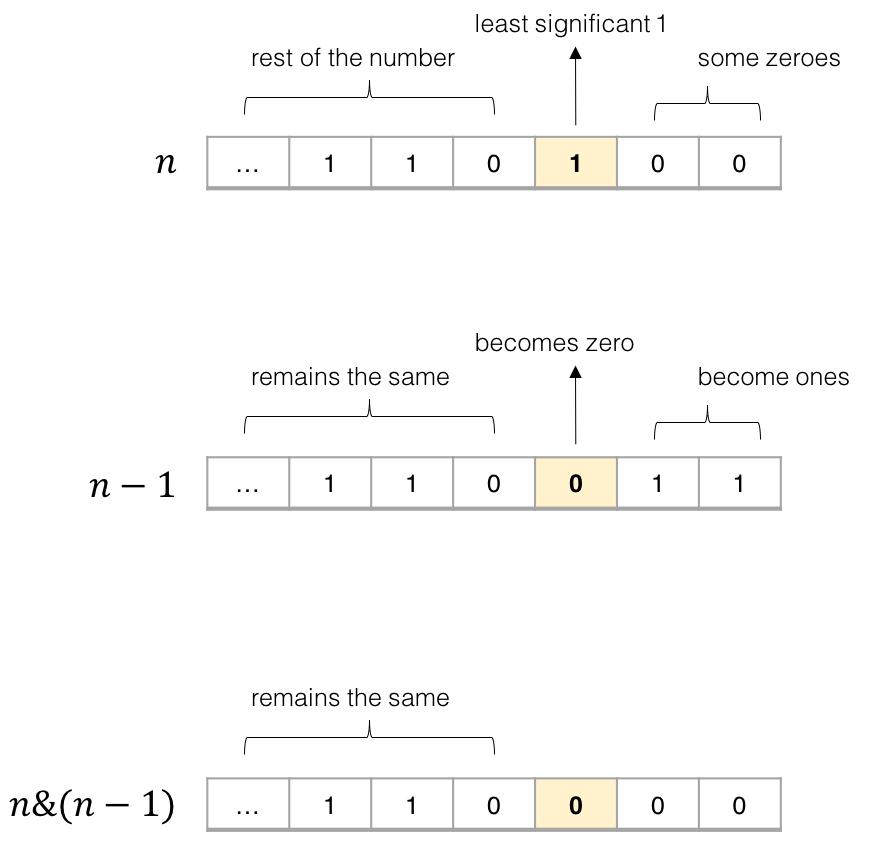
\includegraphics[width=.5\textwidth]{fig/Big_Operations_1.png}
\end{figure}

\subsubsection{计算汉明权重(Hamming Weight)}
\begin{figure}[H]
    \centering
    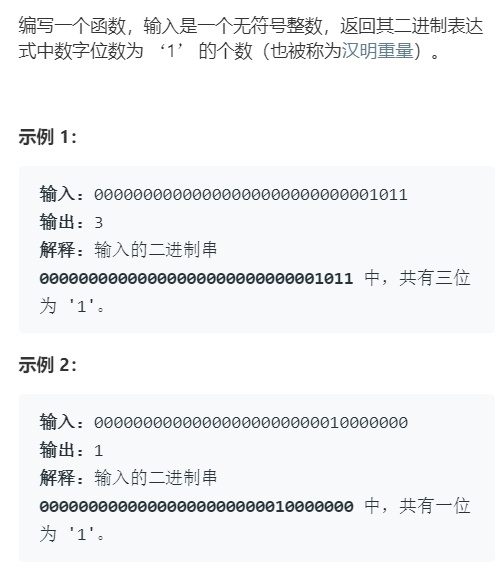
\includegraphics[width=.5\textwidth]{fig/Big_Operations_2.png}
\end{figure}

就是让你返回 n 的二进制表示中有几个 1。因为 n \& (n - 1) 可以消除最后一个 1,所以可以用一个循环不停地消除 1 同时计数,直到 n 变成 0 为止。
\begin{lstlisting}
int hammingWeight(uint32_t n) {
    int res = 0;
    while (n != 0) {
        n = n & (n - 1);
        res++;
    }
    return res;
}
\end{lstlisting}

\subsubsection{判断一个数是不是 2 的指数}
一个数如果是 2 的指数,那么它的二进制表示一定只含有一个 1:
\begin{lstlisting}
2^0 = 1 = 0b0001
2^1 = 2 = 0b0010
2^2 = 4 = 0b0100
\end{lstlisting}

如果使用位运算技巧就很简单了(注意运算符优先级,括号不可以省略):
\begin{lstlisting}
bool isPowerOfTwo(int n) {
    if (n <= 0) return false;
    return (n & (n - 1)) == 0;
}
\end{lstlisting}

\subsection{扩展阅读}
位操作的技巧很多,有一个叫做 Bit Twiddling Hacks 的外国网站收集了几乎所有位操作的黑科技玩法。

\section{烧饼排序}
\url{https://github.com/labuladong/fucking-algorithm/blob/master/%E7%AE%97%E6%B3%95%E6%80%9D%E7%BB%B4%E7%B3%BB%E5%88%97/%E7%83%A7%E9%A5%BC%E6%8E%92%E5%BA%8F.md}

code: \url{computer-basics/codes/pancake_sort.py}

烧饼排序是个很有意思的实际问题:假设盘子上有 n 块面积大小不一的烧饼,你如何用一把锅铲进行若干次翻转,让这些烧饼的大小有序(小的在上,大的在下)?
\begin{figure}[H]
    \centering
    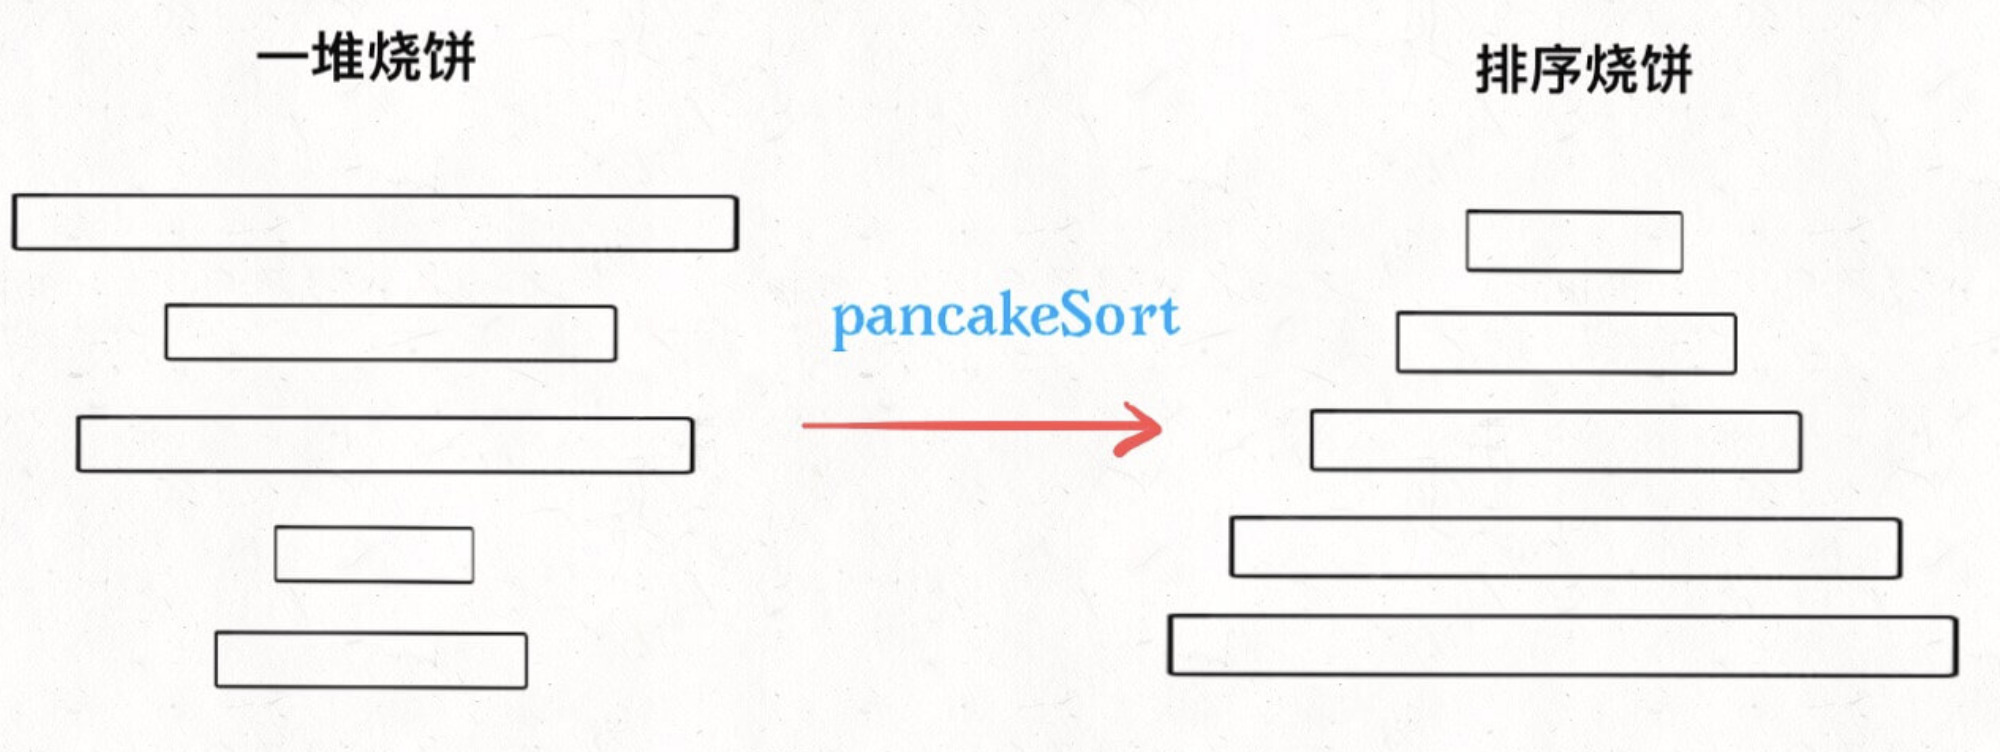
\includegraphics[width=.5\textwidth]{fig/Pancake_Sorting_1.png}
\end{figure}
我们的问题是,如何使用算法得到一个翻转序列,使得烧饼堆变得有序?

首先,需要把这个问题抽象,用数组来表示烧饼堆:
\begin{figure}[H]
    \centering
    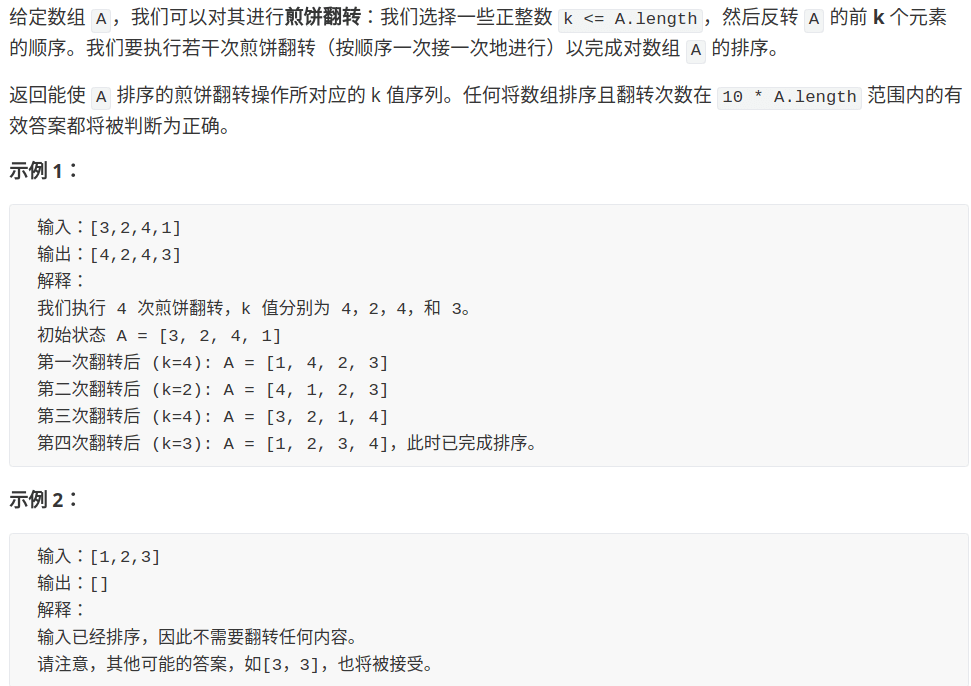
\includegraphics[width=1\textwidth]{fig/Pancake_Sorting_2.png}
\end{figure}
如何解决这个问题呢?这也是需要递归思想的。

\subsection{思路分析}
为什么说这个问题有递归性质呢?比如说我们需要实现这样一个函数:
\begin{lstlisting}
// cakes 是一堆烧饼,函数会将前 n 个烧饼排序
void sort(int[] cakes, int n);
\end{lstlisting}

如果我们找到了前 n 个烧饼中最大的那个,然后设法将这个饼子翻转到最底下,那么,原问题的规模就可以减小,递归调用 pancakeSort(A, n-1) 即可:
\begin{figure}[H]
    \centering
    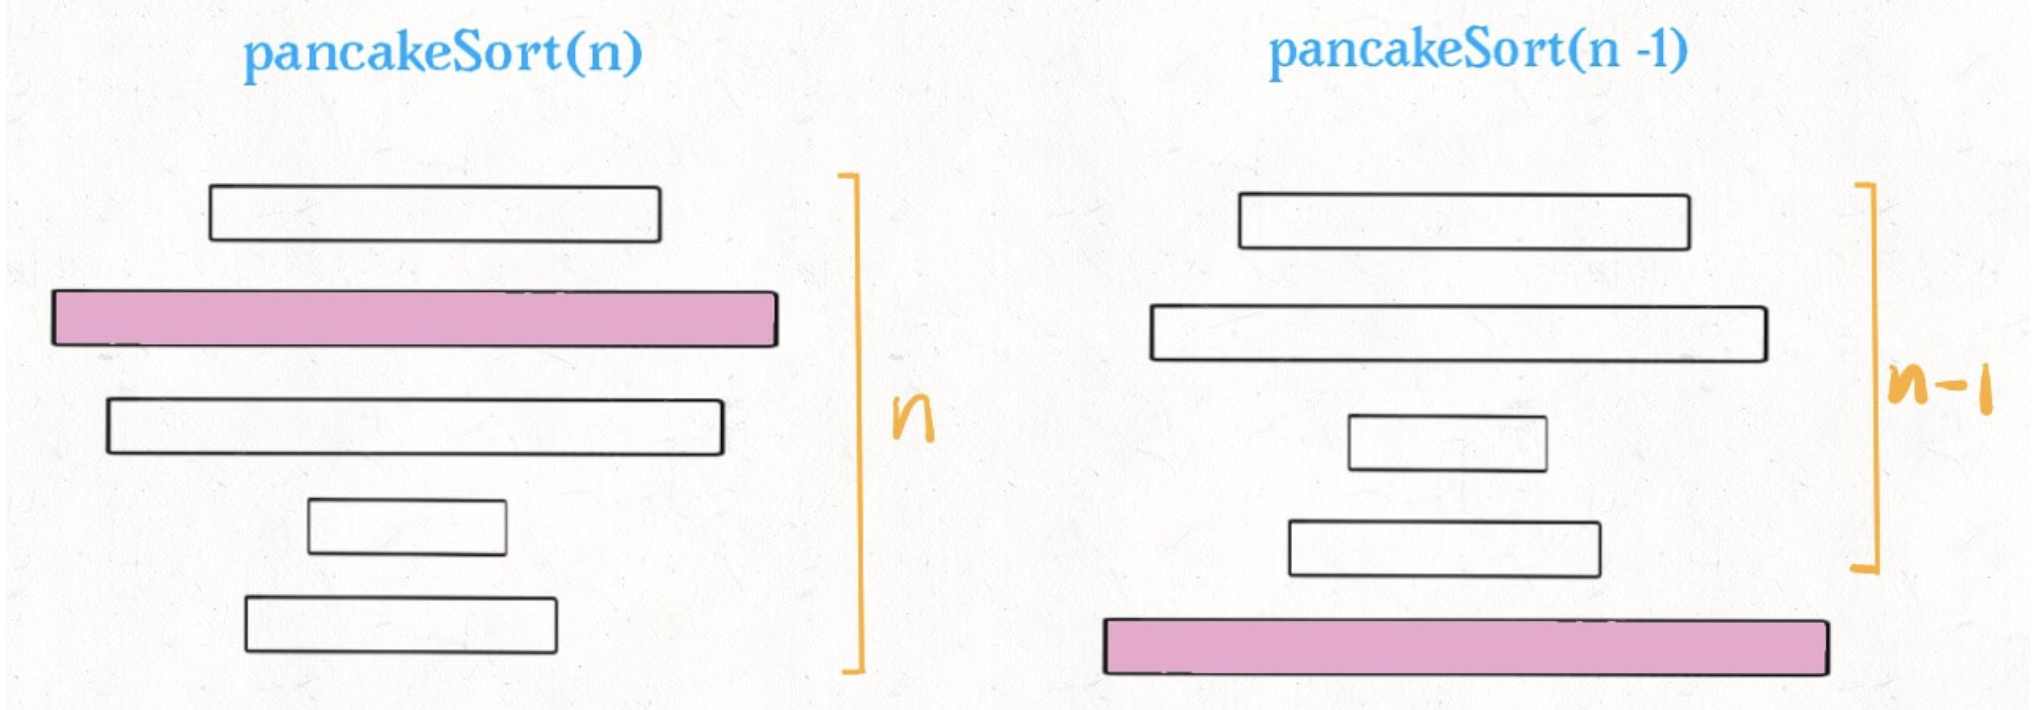
\includegraphics[width=.5\textwidth]{fig/Pancake_Sorting_3.png}
\end{figure}

接下来,对于上面的这 n - 1 块饼,如何排序呢?还是先从中找到最大的一块饼,然后把这块饼放到底下,再递归调用 pancakeSort(A, n-1-1)……

你看,这就是递归性质,总结一下思路就是:
\begin{itemize}
\setlength{\itemsep}{0pt}
\setlength{\parsep}{0pt}
\setlength{\parskip}{0pt}
    \item 找到 n 个饼中最大的那个;
    \item 把这个最大的饼移到最底下;
    \item 递归调用 pancakeSort(A, n - 1);
    \item base case:n == 1 时,排序 1 个饼时不需要翻转
\end{itemize}

那么,最后剩下个问题,如何设法将某块烧饼翻到最后呢?

其实很简单,比如第 3 块饼是最大的,我们想把它换到最后,也就是换到第 n 块。可以这样操作:
\begin{itemize}
\setlength{\itemsep}{0pt}
\setlength{\parsep}{0pt}
\setlength{\parskip}{0pt}
    \item 用锅铲将前 3 块饼翻转一下,这样最大的饼就翻到了最上面;
    \item 用锅铲将前 n 块饼全部翻转,这样最大的饼就翻到了第 n 块,也就是最后一块;
\end{itemize}

以上两个流程理解之后,基本就可以写出解法了,不过题目要求我们写出具体的反转操作序列,这也很简单,只要在每次翻转烧饼时记录下来就行了。

\subsection{代码实现}
只要把上述的思路用代码实现即可,唯一需要注意的是,数组索引从 0 开始,而我们要返回的结果是从 1 开始算的。
\begin{lstlisting}
// 记录反转操作序列
LinkedList<Integer> res = new LinkedList<>();

List<Integer> pancakeSort(int[] cakes) {
    sort(cakes, cakes.length);
    return res;
}

void sort(int[] cakes, int n) {
    // base case
    if (n == 1) return;
    
    // 寻找最大饼的索引
    int maxCake = 0;
    int maxCakeIndex = 0;
    for (int i = 0; i < n; i++)
        if (cakes[i] > maxCake) {
            maxCakeIndex = i;
            maxCake = cakes[i];
        }
    
    // 第一次翻转,将最大饼翻到最上面
    reverse(cakes, 0, maxCakeIndex);
    res.add(maxCakeIndex + 1);
    // 第二次翻转,将最大饼翻到最下面
    reverse(cakes, 0, n - 1);
    res.add(n);

    // 递归调用
    sort(cakes, n - 1);
}

void reverse(int[] arr, int i, int j) {
    while (i < j) {
        int temp = arr[i];
        arr[i] = arr[j];
        arr[j] = temp;
        i++; j--;
    }
}
\end{lstlisting}

通过刚才的详细解释,这段代码应该是很清晰了。

算法的时间复杂度很容易计算,因为递归调用的次数是 n,每次递归调用都需要一次 for 循环,时间复杂度是 O(n),所以总的复杂度是 $O(n^2)$。

最后,我们可以思考一个问题​:按照我们这个思路,得出的操作序列长度应该为​ 2(n - 1),因为每次递归都要进行 2 次翻转并记录操作,总共有 n 层递归,但由于 base case 直接返回结果,不进行翻转,所以最终的操作序列长度应该是固定的 2(n - 1)。

显然,这个结果不是最优的(最短的),比如说一堆煎饼 [3,2,4,1],我们的算法得到的翻转序列是 [3,4,2,3,1,2],但是最快捷的翻转方法应该是 [2,3,4]:
\begin{itemize}
\setlength{\itemsep}{0pt}
\setlength{\parsep}{0pt}
\setlength{\parskip}{0pt}
    \item 初始状态 :[3,2,4,1];
    \item 翻前 2 个:[2,3,4,1];
    \item 翻前 3 个:[4,3,2,1];
    \item 翻前 4 个:[1,2,3,4];
\end{itemize}

如果要求你的算法计算排序烧饼的\textbf{最短操作序列},你该如何计算呢?或者说,解决这种求最优解法的问题,核心思路什么,一定需要使用什么算法技巧呢?

TBD

\section{前缀和技巧}
\subsection{问题背景}
\begin{figure}[H]
    \centering
    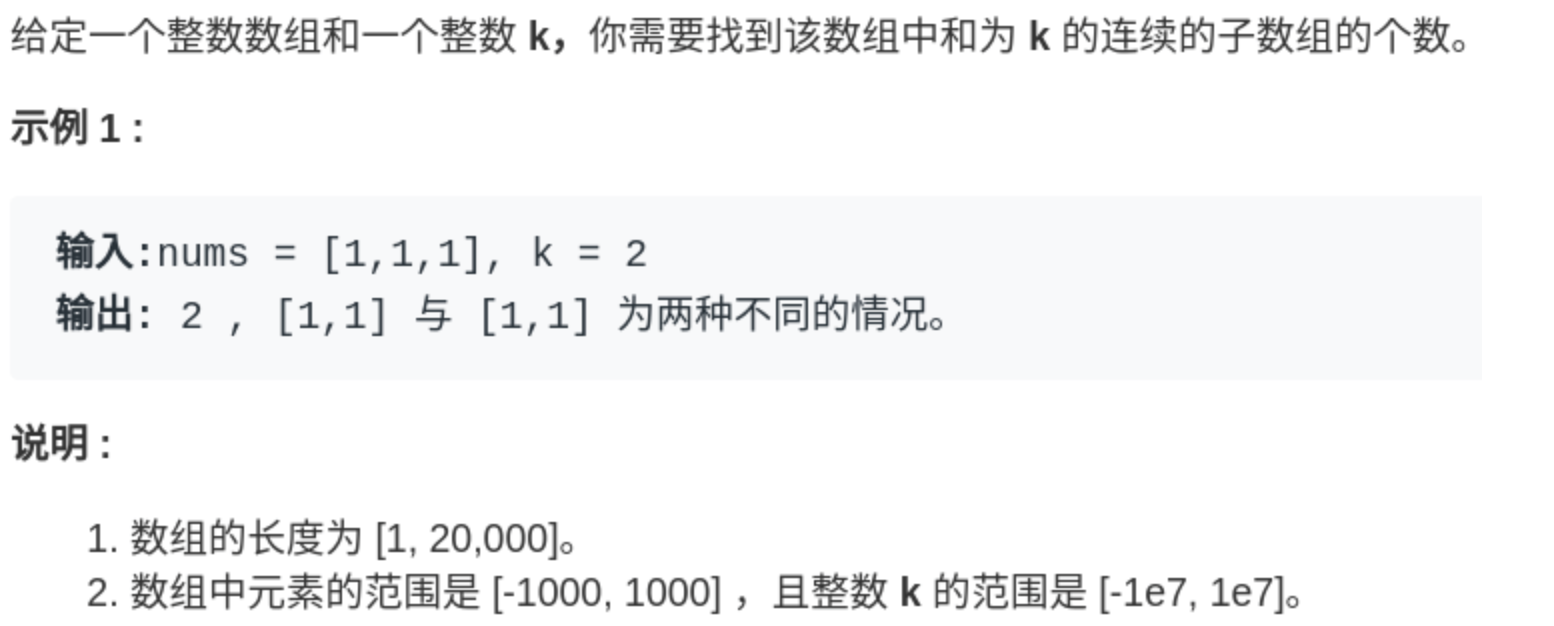
\includegraphics[width=1\textwidth]{fig/Prefix_Tricks_1.png}
\end{figure}

那我把所有子数组都穷举出来,算它们的和,看看谁的和等于 k 不就行了。

关键是,\textbf{如何快速得到某个子数组的和呢},比如说给你一个数组 nums,让你实现一个接口 sum(i, j),这个接口要返回 nums[i..j] 的和,而且会被多次调用,你怎么实现这个接口呢?

因为接口要被多次调用,显然不能每次都去遍历 nums[i..j],有没有一种快速的方法在 O(1) 时间内算出 nums[i..j] 呢?这就需要前缀和技巧了。

\subsection{什么是前缀和}
前缀和的思路是这样的,对于一个给定的数组 nums,我们额外开辟一个前缀和数组进行预处理:
\begin{lstlisting}
int n = nums.length;
// 前缀和数组
int[] preSum = new int[n + 1];
preSum[0] = 0;
for (int i = 0; i < n; i++)
    preSum[i + 1] = preSum[i] + nums[i];
\end{lstlisting}
\begin{figure}[H]
    \centering
    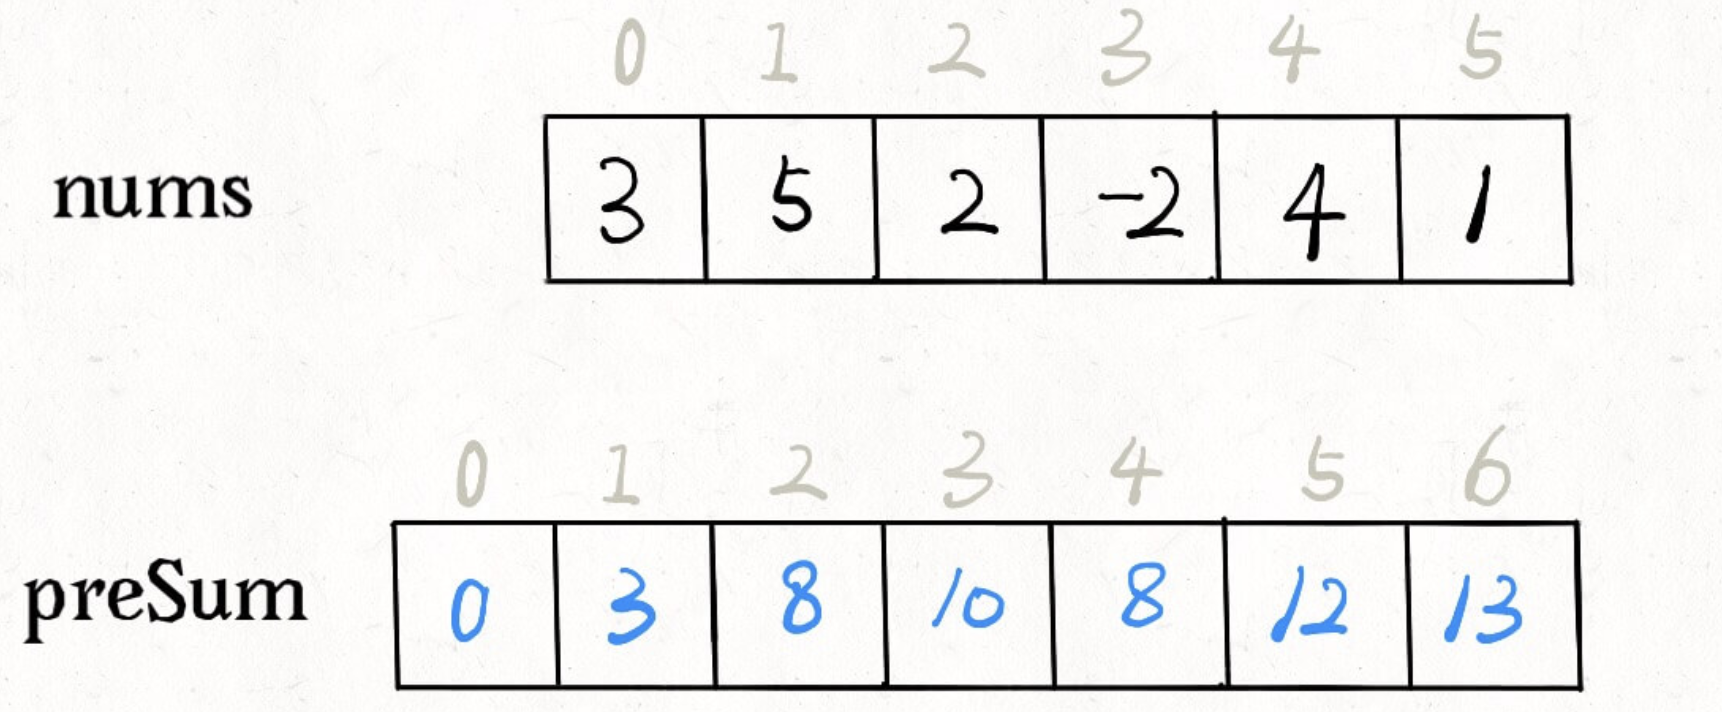
\includegraphics[width=.4\textwidth]{fig/Prefix_Tricks_2.png}
\end{figure}

这个前缀和数组 preSum 的含义也很好理解,preSum[i] 就是 nums[0..i-1] 的和。那么如果我们想求 nums[i..j] 的和,只需要一步操作 preSum[j+1]-preSum[i] 即可,而不需要重新去遍历数组了。

回到这个子数组问题,我们想求有多少个子数组的和为 k,借助前缀和技巧很容易写出一个解法:
\begin{lstlisting}
int subarraySum(int[] nums, int k) {
    int n = nums.length;
    // 构造前缀和
    int[] sum = new int[n + 1];
    sum[0] = 0; 
    for (int i = 0; i < n; i++)
        sum[i + 1] = sum[i] + nums[i];
    
    int ans = 0;
    // 穷举所有子数组
    for (int i = 1; i <= n; i++)
        for (int j = 0; j < i; j++)
            // sum of nums[j..i-1]
            if (sum[i] - sum[j] == k)
                ans++;

    return ans;
}
\end{lstlisting}

这个解法的时间复杂度 $O(N^2)$,空间复杂度 $O(N)$,并不是最优的解法。不过通过这个解法理解了前缀和数组的工作原理之后,可以使用一些巧妙的办法把时间复杂度进一步降低。

\subsection{优化解法}
前面的解法有嵌套的 for 循环:
\begin{lstlisting}
for (int i = 1; i <= n; i++)
    for (int j = 0; j < i; j++)
        if (sum[i] - sum[j] == k)
            ans++;
\end{lstlisting}

第二层 for 循环在干嘛呢?翻译一下就是,在计算,有几个 j 能够使得 sum[i] 和 sum[j] 的差为 k。毎找到一个这样的 j,就把结果加一。

我们可以把 if 语句里的条件判断移项,这样写:
\begin{lstlisting}
if (sum[j] == sum[i] - k)
    ans++;
\end{lstlisting}

优化的思路是:\textbf{我直接记录下有几个 sum[j] 和 sum[i] - k 相等,直接更新结果},就避免了内层的 for 循环。我们可以用哈希表,在记录前缀和的同时记录该前缀和出现的次数。
\begin{lstlisting}
int subarraySum(int[] nums, int k) {
    int n = nums.length;
    // map:前缀和 -> 该前缀和出现的次数
    HashMap<Integer, Integer> preSum = new HashMap<>();
    // base case
    preSum.put(0, 1);

    int ans = 0, sum0_i = 0;
    for (int i = 0; i < n; i++) {
        sum0_i += nums[i];
        // 这是我们想找的前缀和 nums[0..j]
        int sum0_j = sum0_i - k;
        // 如果前面有这个前缀和,则直接更新答案
        if (preSum.containsKey(sum0_j))
            ans += preSum.get(sum0_j);
        // 把前缀和 nums[0..i] 加入并记录出现次数
        preSum.put(sum0_i, 
            preSum.getOrDefault(sum0_i, 0) + 1);
    }
    return ans;
}
\end{lstlisting}

比如说下面这个情况,需要前缀和 8 就能找到和为 k 的子数组了,之前的暴力解法需要遍历数组去数有几个 8,而优化解法借助哈希表可以直接得知有几个前缀和为 8。
\begin{figure}[H]
    \centering
    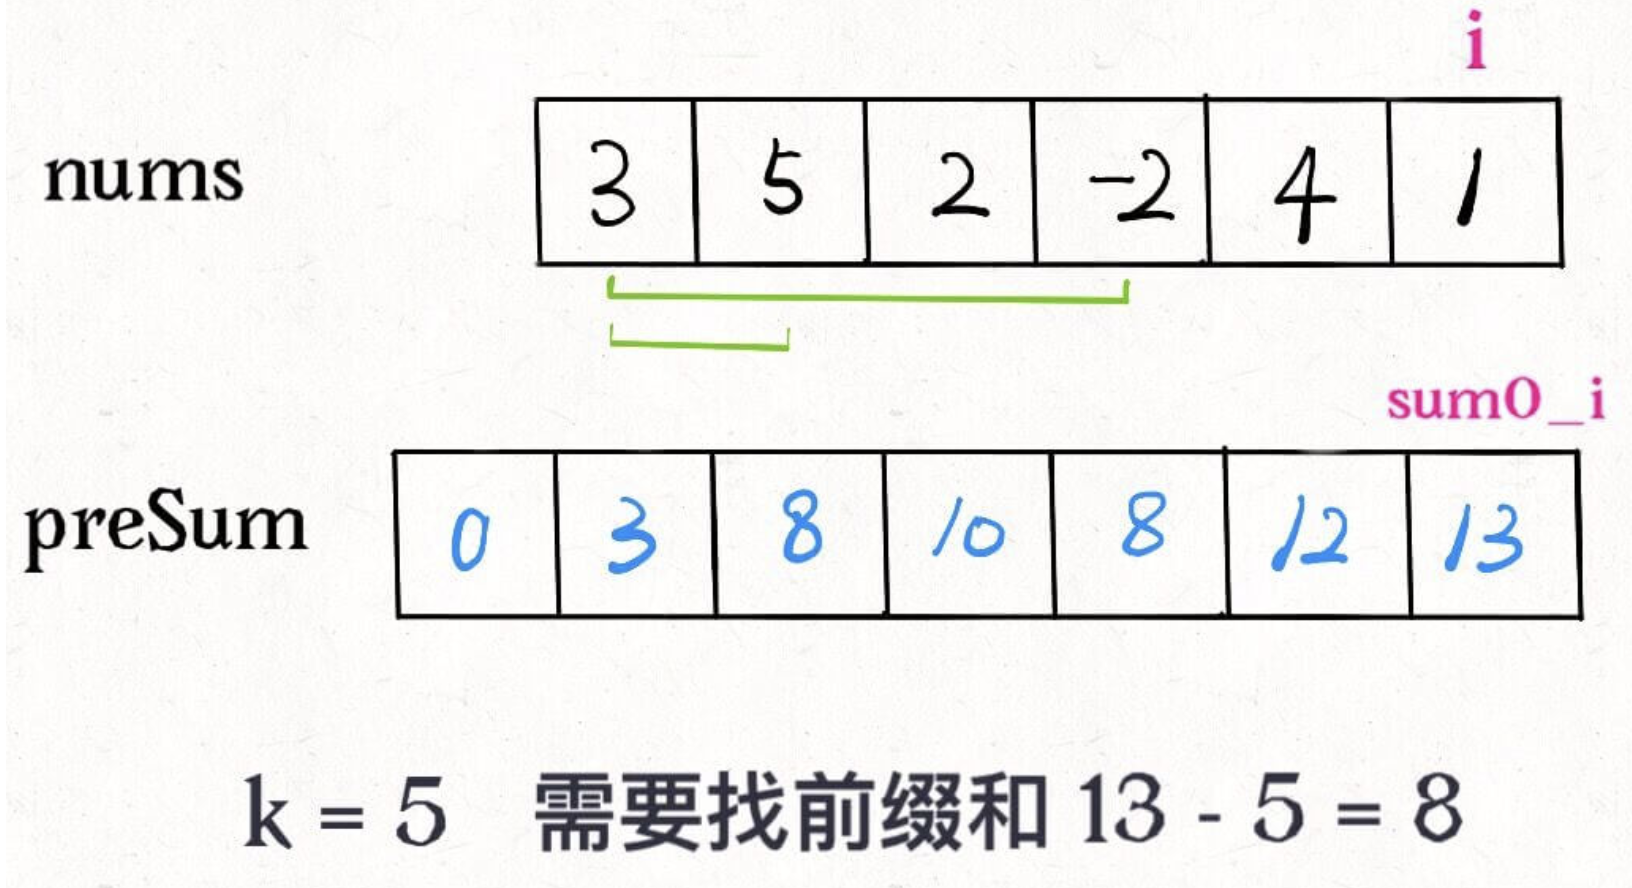
\includegraphics[width=.4\textwidth]{fig/Prefix_Tricks_3.png}
\end{figure}

这样,就把时间复杂度降到了 $O(N)$,是最优解法了。

\subsection{总结}
前缀和不难,却很有用,主要用于处理数组区间的问题。

比如说,让你统计班上同学考试成绩在不同分数段的百分比,也可以利用前缀和技巧:
\begin{lstlisting}
int[] scores; // 存储着所有同学的分数
// 试卷满分 150 分
int[] count = new int[150 + 1]
// 记录每个分数有几个同学
for (int score : scores)
    count[score]++
// 构造前缀和
for (int i = 1; i < count.length; i++)
    count[i] = count[i] + count[i-1];
\end{lstlisting}

这样,给你任何一个分数段,你都能通过前缀和相减快速计算出这个分数段的人数,百分比也就很容易计算了。

但是,稍微复杂一些的算法问题,不止考察简单的前缀和技巧。比如本文探讨的这道题目,就需要借助前缀和的思路做进一步的优化,借助哈希表去除不必要的嵌套循环。可见对题目的理解和细节的分析能力对于算法的优化是至关重要的。

\section{字符串乘法}
\url{https://github.com/labuladong/fucking-algorithm/blob/master/%E7%AE%97%E6%B3%95%E6%80%9D%E7%BB%B4%E7%B3%BB%E5%88%97/%E5%AD%97%E7%AC%A6%E4%B8%B2%E4%B9%98%E6%B3%95.md}

对于比较小的数字,做运算可以直接使用编程语言提供的运算符,但是如果相乘的两个因数非常大,语言提供的数据类型可能就会溢出。一种替代方案就是,运算数以字符串的形式输入,然后模仿我们小学学习的乘法算术过程计算出结果,并且也用字符串表示。

需要注意的是,num1 和 num2 可以非常长,所以不可以把他们直接转成整型然后运算,唯一的思路就是模仿我们手算乘法。

比如说我们手算 123 × 45,应该会这样计算:
\begin{figure}[H]
    \centering
    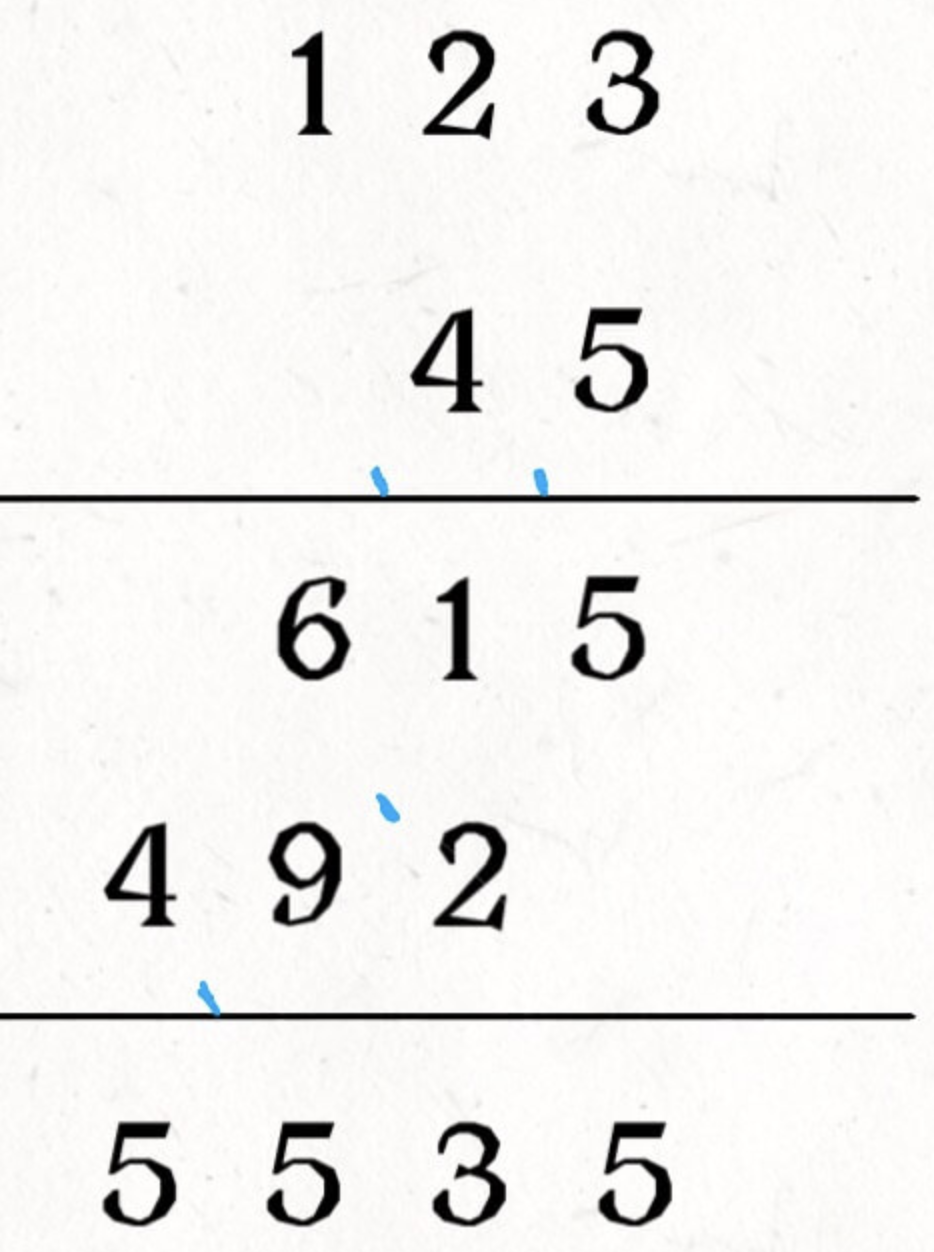
\includegraphics[width=.2\textwidth]{fig/String_Multiply_1.png}
\end{figure}

计算 123 × 5,再计算 123 × 4,最后错一位相加。这个流程恐怕小学生都可以熟练完成,但是你是否能把这个运算过程进一步机械化,写成一套算法指令让没有任何智商的计算机来执行呢?

你看这个简单过程,其中涉及乘法进位,涉及错位相加,还涉及加法进位;而且还有一些不易察觉的问题,比如说两位数乘以两位数,结果可能是四位数,也可能是三位数,你怎么想出一个标准化的处理方式?这就是算法的魅力,如果没有计算机思维,简单的问题可能都没办法自动化处理。

首先,我们这种手算方式还是太「高级」了,我们要再「低级」一点,123 × 5 和 123 × 4 的过程还可以进一步分解,最后再相加。
\begin{figure}[H]
    \centering
    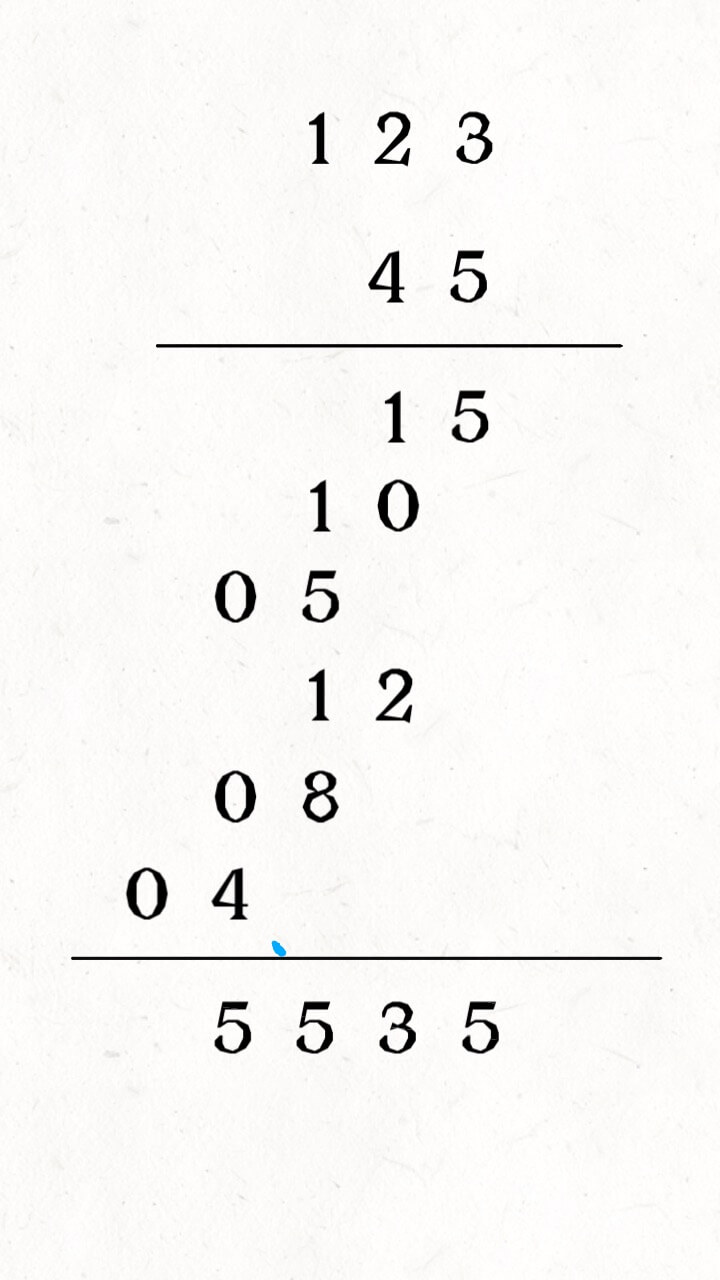
\includegraphics[width=.2\textwidth]{fig/String_Multiply_2.jpg}
\end{figure}

现在 123 并不大,如果是个很大的数字的话,是无法直接计算乘积的。我们可以用一个数组在底下接收相加结果:
\begin{figure}[H]
    \centering
    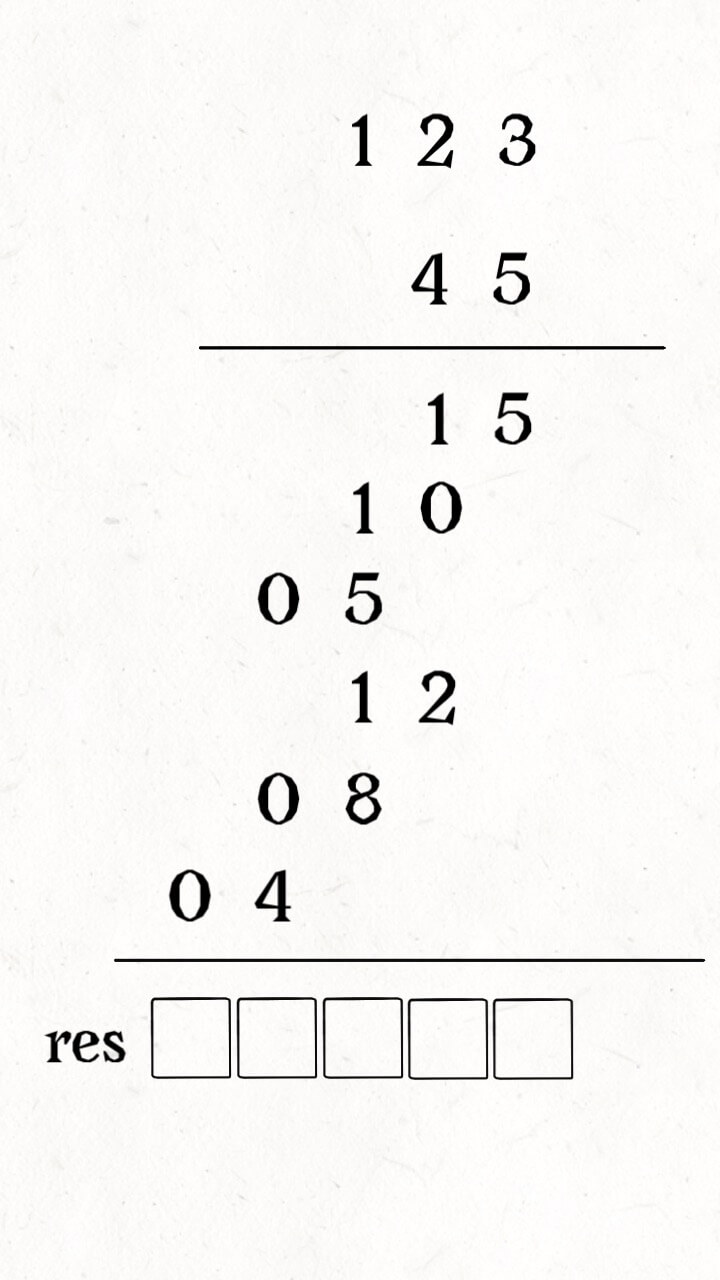
\includegraphics[width=.2\textwidth]{fig/String_Multiply_3.jpg}
\end{figure}

整个计算过程大概是这样,有两个指针 i,j 在 num1 和 num2 上游走,计算乘积,同时将乘积叠加到 res 的正确位置。

其实,细心观察之后就发现,num1[i] 和 num2[j] 的乘积对应的就是 res[i+j] 和 res[i+j+1] 这两个位置。

明白了这一点,就可以用代码模仿出这个计算过程了:
\begin{lstlisting}
string multiply(string num1, string num2) {
    int m = num1.size(), n = num2.size();
    // 结果最多为 m + n 位数
    vector<int> res(m + n, 0);
    // 从个位数开始逐位相乘
    for (int i = m - 1; i >= 0; i--)
        for (int j = n - 1; j >= 0; j--) {
            int mul = (num1[i]-'0') * (num2[j]-'0');
            // 乘积在 res 对应的索引位置
            int p1 = i + j, p2 = i + j + 1;
            // 叠加到 res 上
            int sum = mul + res[p2];
            res[p2] = sum % 10;
            res[p1] += sum / 10;
        }
    // 结果前缀可能存的 0(未使用的位)
    int i = 0;
    while (i < res.size() && res[i] == 0)
        i++;
    // 将计算结果转化成字符串
    string str;
    for (; i < res.size(); i++)
        str.push_back('0' + res[i]);
    
    return str.size() == 0 ? "0" : str;
}
\end{lstlisting}

至此,字符串乘法算法就完成了。

\section{信封嵌套问题}
\url{https://github.com/labuladong/fucking-algorithm/blob/master/%E7%AE%97%E6%B3%95%E6%80%9D%E7%BB%B4%E7%B3%BB%E5%88%97/%E4%BF%A1%E5%B0%81%E5%B5%8C%E5%A5%97%E9%97%AE%E9%A2%98.md}

信封嵌套问题需要先按特定的规则排序,之后就转换为一个 最长递增子序列问题,可以用前文 二分查找详解 的技巧来解决了。

\subsection{题目概述}
信封嵌套问题是个很有意思且经常出现在生活中的问题,先看下题目:
\begin{figure}[H]
    \centering
    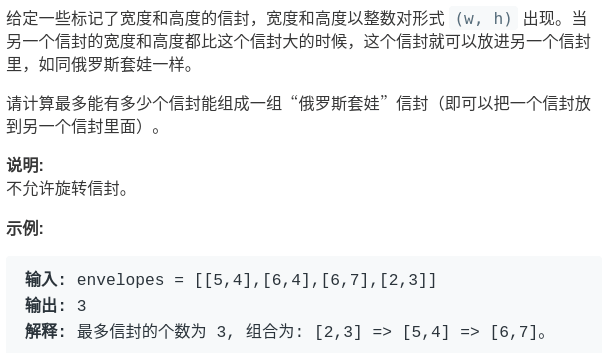
\includegraphics[width=1\textwidth]{fig/Envelope_Packing_1.png}
\end{figure}

这道题目其实是最长递增子序列(Longes Increasing Subsequence,简写为 LIS)的一个变种,因为很显然,每次合法的嵌套是大的套小的,相当于找一个最长递增的子序列,其长度就是最多能嵌套的信封个数。

但是难点在于,标准的 LIS 算法只能在数组中寻找最长子序列,而我们的信封是由 (w, h) 这样的二维数对形式表示的,如何把 LIS 算法运用过来呢?
\begin{figure}[H]
    \centering
    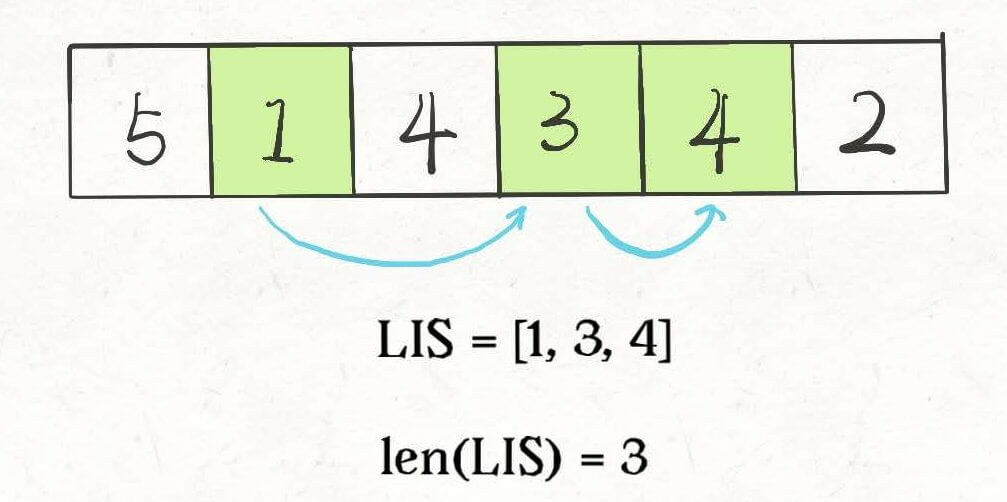
\includegraphics[width=.4\textwidth]{fig/Envelope_Packing_2.jpg}
\end{figure}

读者也许会想,通过 w × h 计算面积,然后对面积进行标准的 LIS 算法。但是稍加思考就会发现这样不行,比如 1 × 10 大于 3 × 3,但是显然这样的两个信封是无法互相嵌套的。

\subsection{解法}
这道题的解法是比较巧妙的:

\textbf{先对宽度 w 进行升序排序,如果遇到 w 相同的情况,则按照高度 h 降序排序。之后把所有的 h 作为一个数组,在这个数组上计算 LIS 的长度就是答案。}

画个图理解一下,先对这些数对进行排序:
\begin{figure}[H]
    \centering
    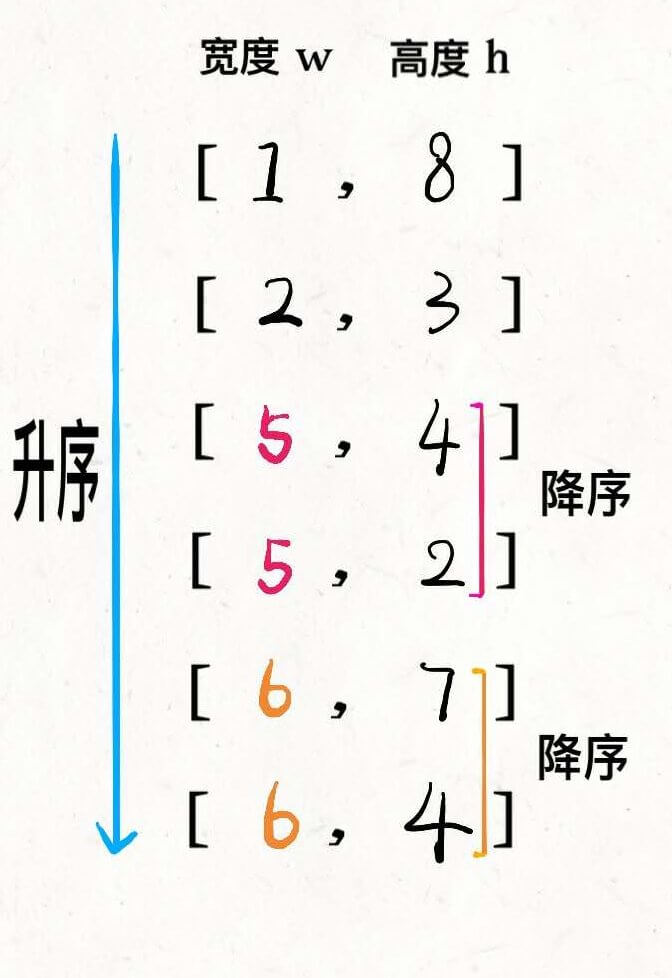
\includegraphics[width=.2\textwidth]{fig/Envelope_Packing_3.jpg}
\end{figure}

然后在 h 上寻找最长递增子序列:
\begin{figure}[H]
    \centering
    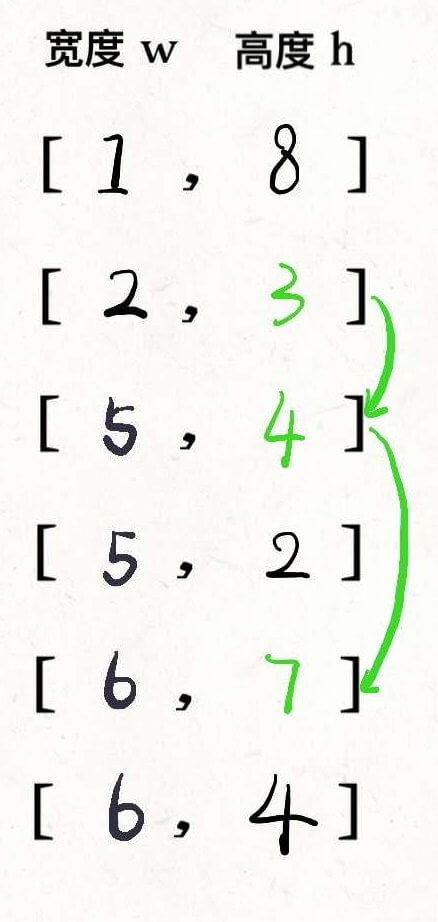
\includegraphics[width=.2\textwidth]{fig/Envelope_Packing_4.jpg}
\end{figure}

这个子序列就是最优的嵌套方案。

这个解法的关键在于,对于宽度 w 相同的数对,要对其高度 h 进行降序排序。因为两个宽度相同的信封不能相互包含的,逆序排序保证在 w 相同的数对中最多只选取一个。
\begin{lstlisting}
// envelopes = [[w, h], [w, h]...]
public int maxEnvelopes(int[][] envelopes) {
    int n = envelopes.length;
    // 按宽度升序排列,如果宽度一样,则按高度降序排列
    Arrays.sort(envelopes, new Comparator<int[]>() 
    {
        public int compare(int[] a, int[] b) {
            return a[0] == b[0] ? 
                b[1] - a[1] : a[0] - b[0];
        }
    });
    // 对高度数组寻找 LIS
    int[] height = new int[n];
    for (int i = 0; i < n; i++)
        height[i] = envelopes[i][1];

    return lengthOfLIS(height);
}
\end{lstlisting}

此算法的时间复杂度为 $O(NlogN)$,因为排序和计算 LIS 各需要 $O(NlogN)$ 的时间。

空间复杂度为 $O(N)$,因为计算 LIS 的函数中需要一个 top 数组。

\subsection{拓展}
其实这种问题还可以拓展到三维,比如说现在不是让你嵌套信封,而是嵌套箱子,每个箱子有长宽高三个维度,请你算算最多能嵌套几个箱子?

我们可能会这样想,先把前两个维度(长和宽)按信封嵌套的思路求一个嵌套序列,最后在这个序列的第三个维度(高度)找一下 LIS,应该能算出答案。

实际上,这个思路是错误的。这类问题叫做「偏序问题」,上升到三维会使难度巨幅提升,需要借助一种高级数据结构「树状数组」,有兴趣的读者可以自行搜索。

\section{洗牌算法}
\url{https://github.com/labuladong/fucking-algorithm/blob/master/%E7%AE%97%E6%B3%95%E6%80%9D%E7%BB%B4%E7%B3%BB%E5%88%97/%E6%B4%97%E7%89%8C%E7%AE%97%E6%B3%95.md}

我知道大家会各种花式排序算法,但是如果叫你打乱一个数组,你是否能做到胸有成竹?即便你拍脑袋想出一个算法,怎么证明你的算法就是正确的呢?乱序算法不像排序算法,结果唯一可以很容易检验,因为「乱」可以有很多种,你怎么能证明你的算法是「真的乱」呢?

所以我们面临两个问题:什么叫做「真的乱」?设计怎样的算法来打乱数组才能做到「真的乱」?

这种算法称为「随机乱置算法」或者「洗牌算法」。

本文分两部分,第一部分详解最常用的洗牌算法。因为该算法的细节容易出错,且存在好几种变体,虽有细微差异但都是正确的,所以本文要介绍一种简单的通用思想保证你写出正确的洗牌算法。第二部分讲解使用「蒙特卡罗方法」来检验我们的打乱结果是不是真的乱。蒙特卡罗方法的思想不难,但是实现方式也各有特点的。

\subsection{洗牌算法}
此类算法都是靠随机选取元素交换来获取随机性,直接看代码(伪码),该算法有 4 种形式,都是正确的:

\begin{lstlisting}
// 得到一个在闭区间 [min, max] 内的随机整数
int randInt(int min, int max);

// 第一种写法
void shuffle(int[] arr) {
    int n = arr.length();
    /******** 区别只有这两行 ********/
    for (int i = 0 ; i < n; i++) {
        // 从 i 到最后随机选一个元素
        int rand = randInt(i, n - 1);
        /*************************/
        swap(arr[i], arr[rand]);
    }
}

// 第二种写法
    for (int i = 0 ; i < n - 1; i++)
        int rand = randInt(i, n - 1);

// 第三种写法
    for (int i = n - 1 ; i >= 0; i--)
        int rand = randInt(0, i);

// 第四种写法
    for (int i = n - 1 ; i > 0; i--)
        int rand = randInt(0, i);
\end{lstlisting}

分析洗牌算法正确性的准则:\textbf{产生的结果必须有 n! 种可能,否则就是错误的}。这个很好解释,因为一个长度为 n 的数组的全排列就有 n! 种,也就是说打乱结果总共有 n! 种。算法必须能够反映这个事实,才是正确的。

我们先用这个准则分析一下第一种写法的正确性:
\begin{lstlisting}
// 假设传入这样一个 arr
int[] arr = {1,3,5,7,9};

void shuffle(int[] arr) {
    int n = arr.length(); // 5
    for (int i = 0 ; i < n; i++) {
        int rand = randInt(i, n - 1);
        swap(arr[i], arr[rand]);
    }
}
\end{lstlisting}

for 循环第一轮迭代时,i = 0,rand 的取值范围是 [0, 4],有 5 个可能的取值。
\begin{figure}[H]
    \centering
    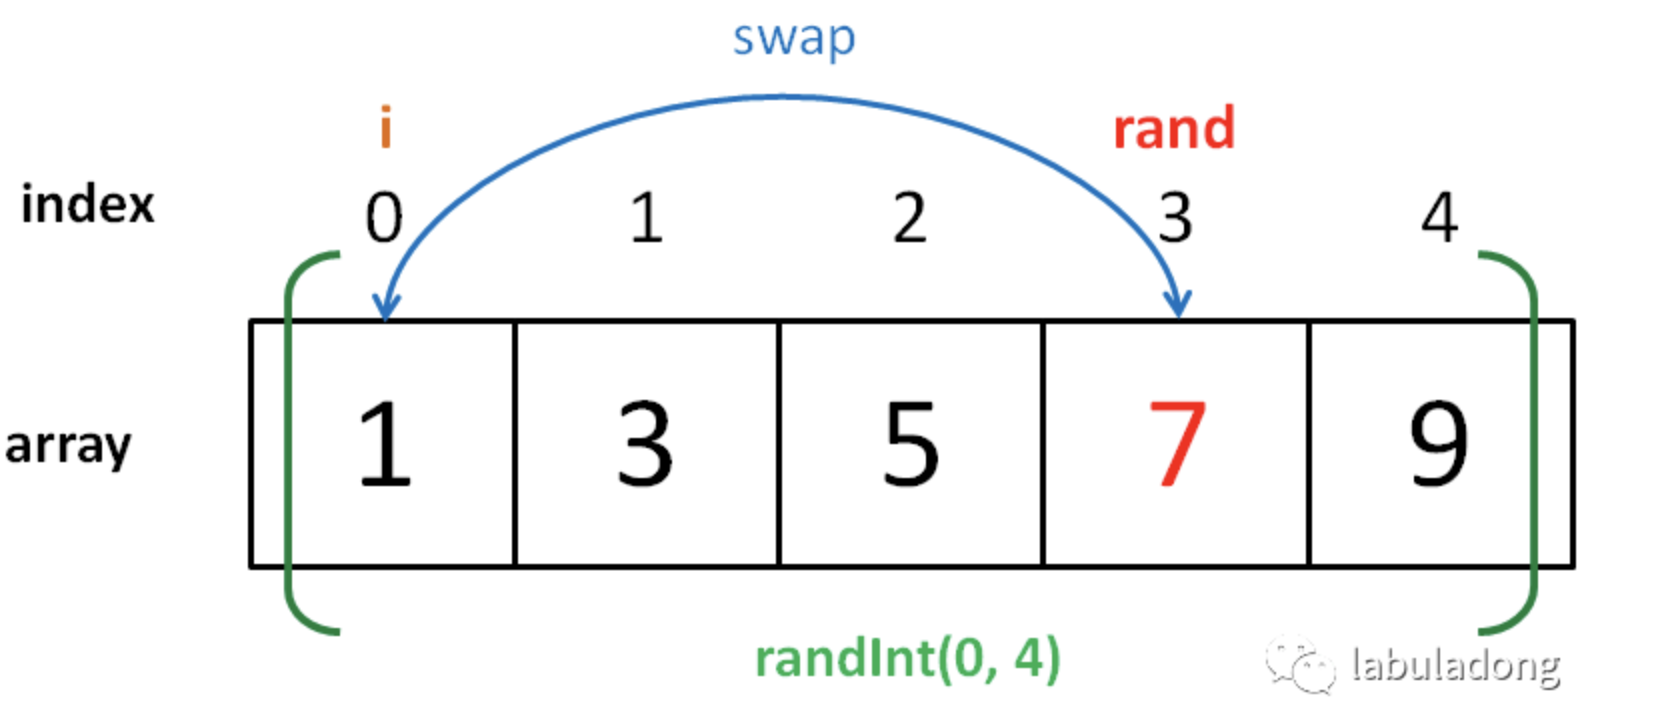
\includegraphics[width=.6\textwidth]{fig/shuffle_algorithm_1.png}
\end{figure}

for 循环第二轮迭代时,i = 1,rand 的取值范围是 [1, 4],有 4 个可能的取值。
\begin{figure}[H]
    \centering
    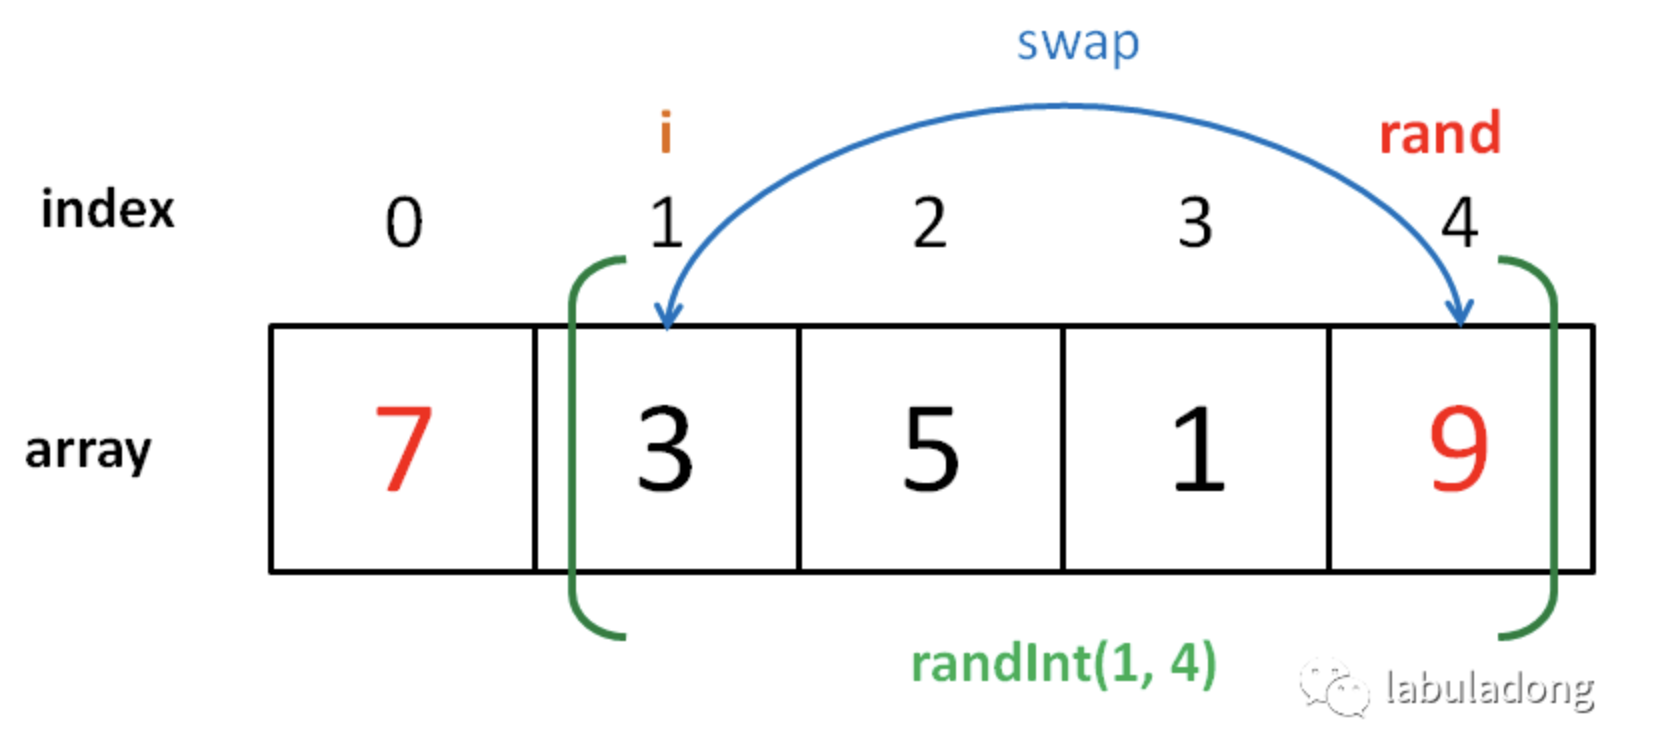
\includegraphics[width=.6\textwidth]{fig/shuffle_algorithm_2.png}
\end{figure}

后面以此类推,直到最后一次迭代,i = 4,rand 的取值范围是 [4, 4],只有 1 个可能的取值。
\begin{figure}[H]
    \centering
    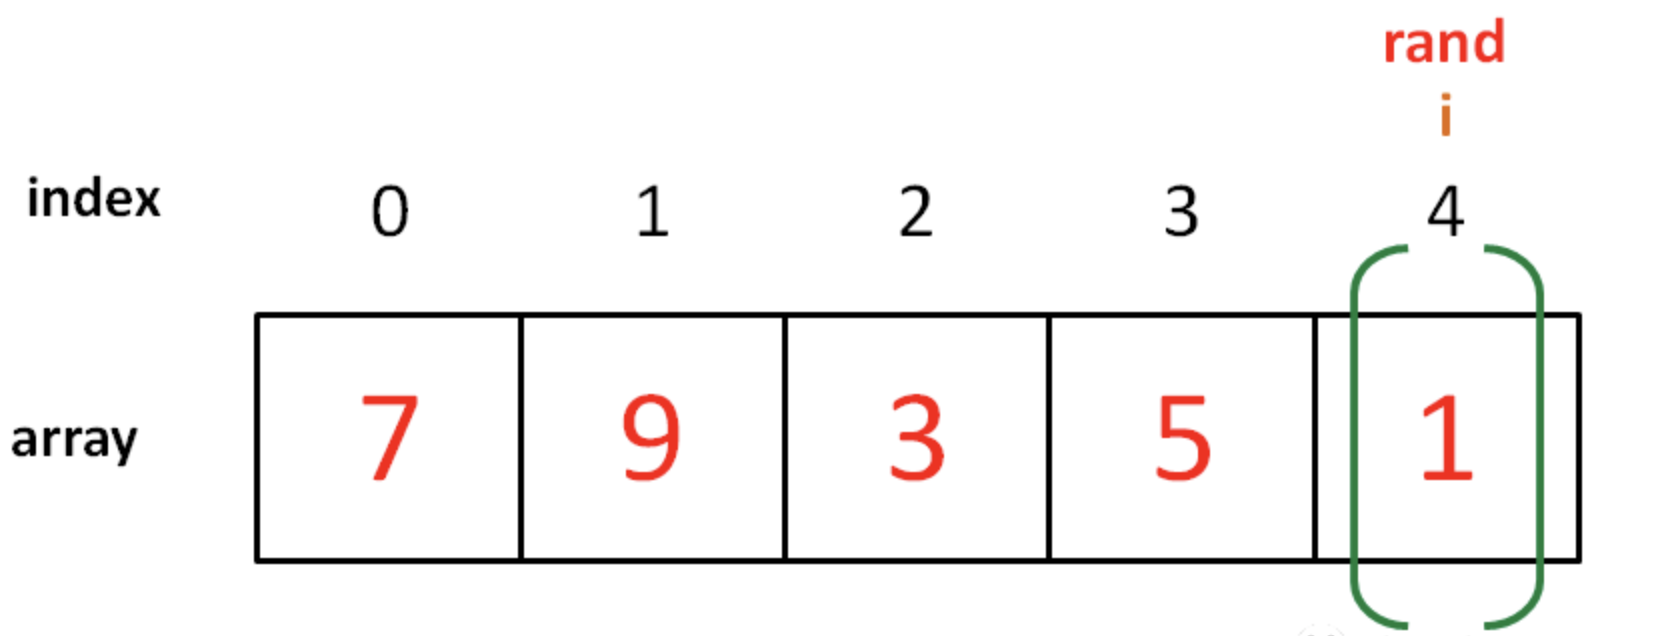
\includegraphics[width=.6\textwidth]{fig/shuffle_algorithm_3.png}
\end{figure}

可以看到,整个过程产生的所有可能结果有 $n! = 5! = 5*4*3*2*1$ 种,所以这个算法是正确的。

分析第二种写法,前面的迭代都是一样的,少了一次迭代而已。所以最后一次迭代时 i = 3,rand 的取值范围是 [3, 4],有 2 个可能的取值。
\begin{lstlisting}
// 第二种写法
// arr = {1,3,5,7,9}, n = 5
    for (int i = 0 ; i < n - 1; i++)
        int rand = randInt(i, n - 1);
\end{lstlisting}

所以整个过程产生的所有可能结果仍然有 $5*4*3*2 = 5! = n! $种,因为乘以 1 可有可无嘛。所以这种写法也是正确的。

如果以上内容你都能理解,那么你就能发现第三种写法就是第一种写法,只是将数组从后往前迭代而已;第四种写法是第二种写法从后往前来。所以它们都是正确的。

如果读者思考过洗牌算法,可能会想出如下的算法,但是\textbf{这种写法是错误的}:
\begin{lstlisting}
void shuffle(int[] arr) {
    int n = arr.length();
    for (int i = 0 ; i < n; i++) {
        // 每次都从闭区间 [0, n-1]
        // 中随机选取元素进行交换
        int rand = randInt(0, n - 1);
        swap(arr[i], arr[rand]);
    }
}
\end{lstlisting}

现在你应该明白这种写法为什么会错误了。\textbf{因为这种写法得到的所有可能结果有 $n^n$ 种,而不是 $n!$ 种,而且 $n^n$ 不可能是 $n!$ 的整数倍}。

比如说 arr = [1,2,3],正确的结果应该有 $3!= 6$ 种可能,而这种写法总共有 $3^3 = 27$ 种可能结果。因为 27 不能被 6 整除,所以一定有某些情况被「偏袒」了,也就是说某些情况出现的概率会大一些,所以这种打乱结果不算「真的乱」。

上面我们从直觉上简单解释了洗牌算法正确的准则,没有数学证明,我想大家也懒得证明。对于概率问题我们可以使用「蒙特卡罗方法」进行简单验证。

\subsection{蒙特卡罗方法验证正确性}
洗牌算法,或者说随机乱置算法的正确性衡量标准是:\textbf{对于每种可能的结果出现的概率必须相等,也就是说要足够随机}。

如果不用数学严格证明概率相等,可以用蒙特卡罗方法近似地估计出概率是否相等,结果是否足够随机。

记得高中有道数学题:往一个正方形里面随机打点,这个正方形里紧贴着一个圆,告诉你打点的总数和落在圆里的点的数量,让你计算圆周率。这其实就是利用了蒙特卡罗方法:当打的点足够多的时候,点的数量就可以近似代表图形的面积。通过面积公式,由正方形和圆的面积比值是可以很容易推出圆周率的。当然打的点越多,算出的圆周率越准确,充分体现了大力出奇迹的真理。

类似的,我们可以对同一个数组进行一百万次洗牌,统计各种结果出现的次数,把频率作为概率,可以很容易看出洗牌算法是否正确。整体思想很简单,不过实现起来也有些技巧的,下面简单分析几种实现思路。

\textbf{第一种思路},我们把数组 arr 的所有排列组合都列举出来,做成一个直方图(假设 arr = [1,2,3]):
\begin{figure}[H]
    \centering
    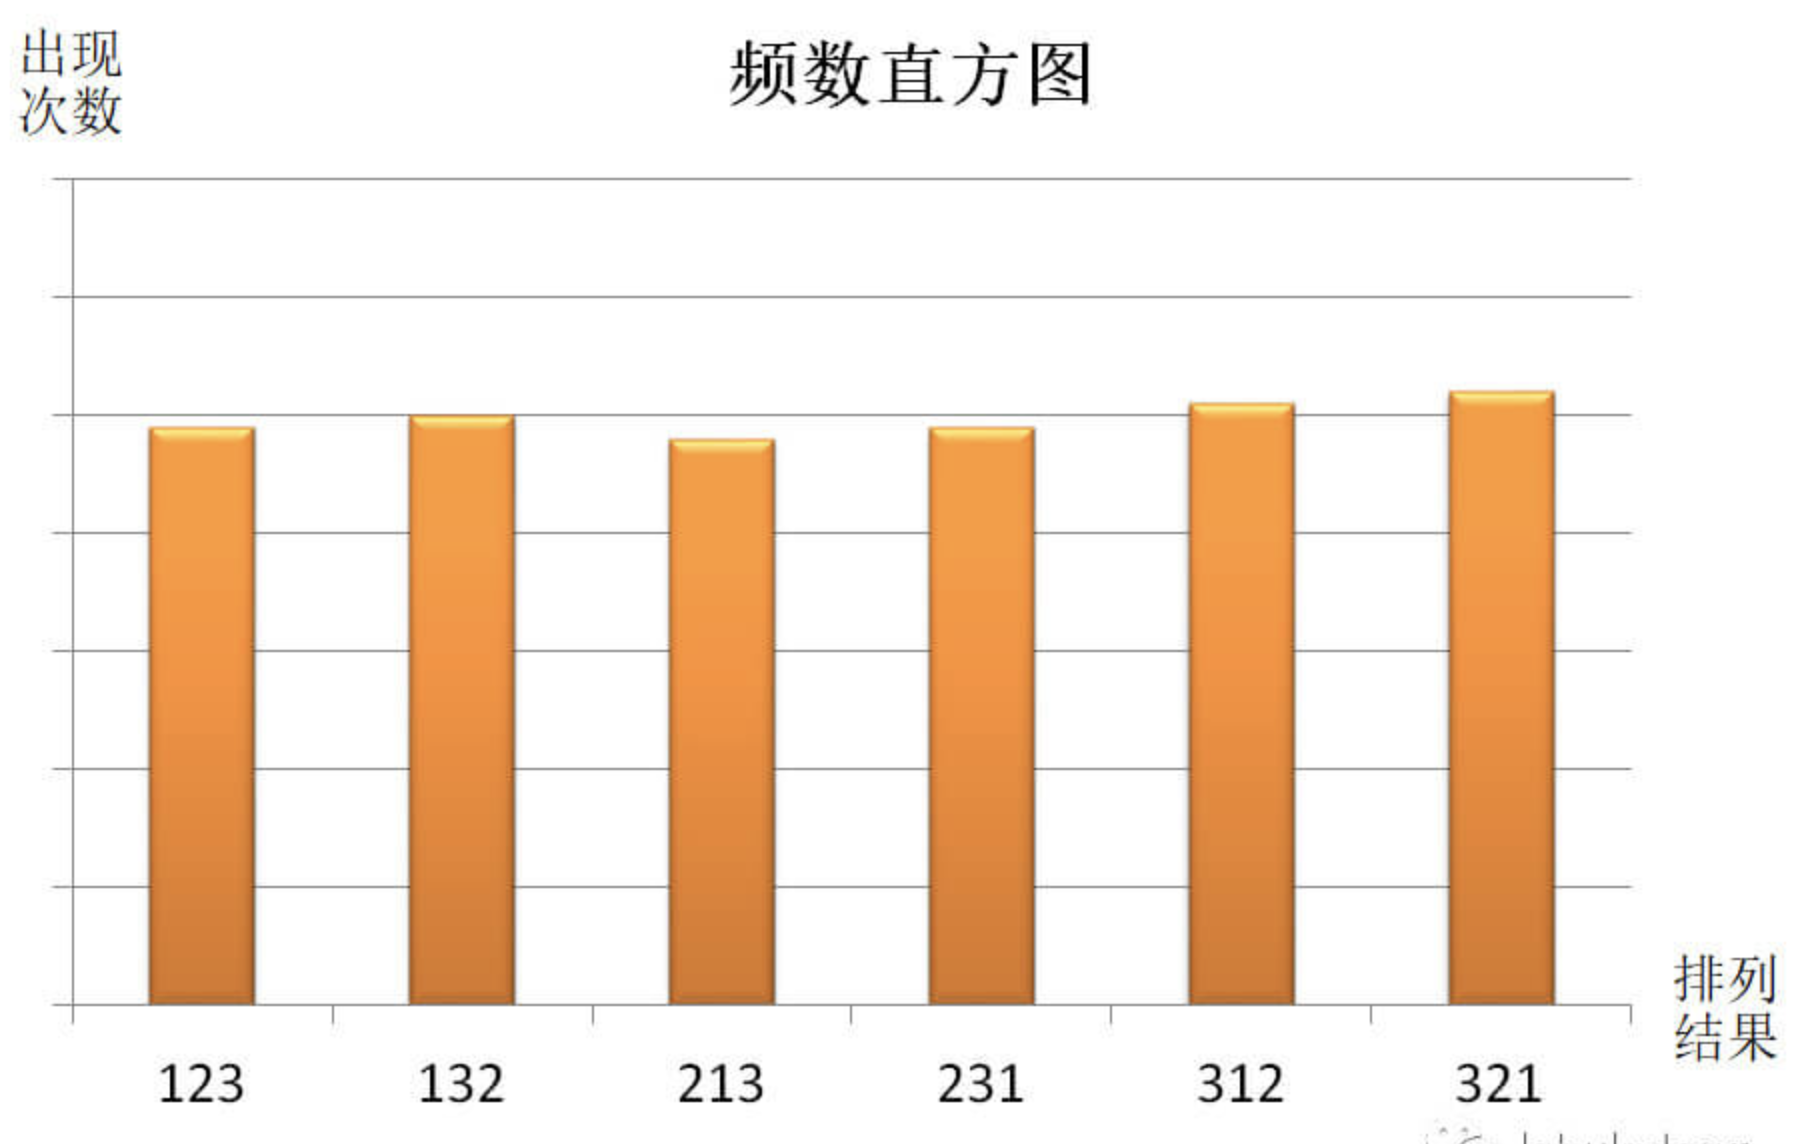
\includegraphics[width=.6\textwidth]{fig/shuffle_algorithm_4.png}
\end{figure}

每次进行洗牌算法后,就把得到的打乱结果对应的频数加一,重复进行 100 万次,如果每种结果出现的总次数差不多,那就说明每种结果出现的概率应该是相等的。写一下这个思路的伪代码:
\begin{lstlisting}
void shuffle(int[] arr);

// 蒙特卡罗
int N = 1000000;
HashMap count; // 作为直方图
for (i = 0; i < N; i++) {
    int[] arr = {1,2,3};
    shuffle(arr);
    // 此时 arr 已被打乱
    count[arr] += 1;
}
for (int feq : count.values()) 
    print(feq / N + " "); // 频率
\end{lstlisting}
这种检验方案是可行的,不过可能有读者会问,arr 的全部排列有 n! 种(n 为 arr 的长度),如果 n 比较大,那岂不是空间复杂度爆炸了?

是的,不过作为一种验证方法,我们不需要 n 太大,一般用长度为 5 或 6 的 arr 试下就差不多了吧,因为我们只想比较概率验证一下正确性而已。

\textbf{第二种思路},可以这样想,arr 数组中全都是 0,只有一个 1。我们对 arr 进行 100 万次打乱,记录每个索引位置出现 1 的次数,如果每个索引出现的次数差不多,也可以说明每种打乱结果的概率是相等的。
\begin{lstlisting}
void shuffle(int[] arr);

// 蒙特卡罗方法
int N = 1000000;    
int[] arr = {1,0,0,0,0};
int[] count = new int[arr.length];
for (int i = 0; i < N; i++) {
    shuffle(arr); // 打乱 arr
    for (int j = 0; j < arr.length; j++) 
        if (arr[j] == 1) {
            count[j]++;
            break;
        }
}
for (int feq : count) 
    print(feq / N + " "); // 频率
\end{lstlisting}

这种思路也是可行的,而且避免了阶乘级的空间复杂度,但是多了嵌套 for 循环,时间复杂度高一点。不过由于我们的测试数据量不会有多大,这些问题都可以忽略。

另外,细心的读者可能发现一个问题,上述两种思路声明 arr 的位置不同,一个在 for 循环里,一个在 for 循环之外。其实效果都是一样的,因为我们的算法总要打乱 arr,所以 arr 的顺序并不重要,只要元素不变就行。

\subsection{总结}
本文第一部分介绍了洗牌算法(随机乱置算法),通过一个简单的分析技巧证明了该算法的四种正确形式,并且分析了一种常见的错误写法,相信你一定能够写出正确的洗牌算法了。

第二部分写了洗牌算法正确性的衡量标准,即每种随机结果出现的概率必须相等。如果我们不用严格的数学证明,可以通过蒙特卡罗方法大力出奇迹,粗略验证算法的正确性。蒙特卡罗方法也有不同的思路,不过要求不必太严格,因为我们只是寻求一个简单的验证。




%\printbibliography
\bibliography{../ref}
\bibliographystyle{IEEEtran}
\end{document}